\documentclass{article}
\usepackage{csvsimple}
\usepackage{amsmath}
\usepackage{amssymb}
\usepackage{graphicx}
\usepackage{hyperref}
\usepackage{wrapfig}
\usepackage[utf8]{inputenc}
\usepackage{graphicx}
\usepackage[
backend=biber,
style=alphabetic,
]{biblatex}
\usepackage{multicol}
\usepackage{setspace}
\usepackage{datetime}
\usepackage{flushend} % For end of document
\usepackage[super]{nth}
\usepackage{enumitem} % to use custom enumration

% \addbibresource{rcheruiyotrefs.bib} %Imports bibliography file
\addbibresource{refs.bib}

\begin{document}

%insert your content here..

\section{Student content}
% added \usepackage[utf8]{inputenc} to Assignment3-git.tex
% added \usepackage{graphicx} to Assignment3-git.tex
% appended {IEEEtran} to \documentclass{article} in Assignment3-git.tex
% removed the \ { } characters surrounding KoraComments
% changed lines below
%  \bibliographystyle{IEEEtran}
%  \bibliography{refs}
% to \addbibresource{refs.bib} added to Assignment3-git.tex
% would include \printbibliography, however, I do not know what to cite for them
\section{Fall 2024 Student Content}



\section{Introduction : Sahil Thapa}
I am Sahil Thapa, a PhD in Computer Science. My advisor, Dr. Oluwatosin Oluwadare, guides my research, and I also serve as a graduate research assistant in his bioinformatics lab. My research focuses on utilizing deep learning and artificial intelligence to develop bioinformatics tools, with a current emphasis on splice site detection methods.\\

From a young age, I have enjoyed walking and traveling, a passion instilled in me by my maternal uncle. He often took me to rivers and hills, where we would sit and talk, fostering my love for trekking. I have explored many beautiful places in Nepal, including the Annapurna Mountain Range and the Langtang Circuit. My favorite films are "The Legend of 1900" and "The Forrest Gump."

\begin{figure}[h!]
    \centering
    \includegraphics[width=0.5\linewidth]{images/Sahil_Thapa.jpg}
    \caption{Caption}
    \label{fig:enter-label}
\end{figure}

\section{Output of CNNSplice: Robust models for splice site prediction using convolutional neural networks.}
I explored the following Git repository related to my research: https://github.com/OluwadareLab/CNNSplice.git\\

CNNSplice is a set of deep convolutional neural network models designed for splice site prediction. Developed at the University of Colorado Colorado Springs, CNNSplice aims to efficiently predict true and false splice sites using robust machine learning techniques.

\subsection{test\_logfile\_metrics}
These are Output\_logfile Results of CNNModel.\\
$\{'precision': 0.9027834069851564, 'recall': 0.9206222222222222, 'f1': 0.9111579557303049, 'class_accuracy': 0.9318666666666666, 'accuracy': 0.9318666458129883\}$\\

$\{'precision': 0.9273229649052265, 'recall': 0.9525333333333332, 'f1': 0.9389124679859917, 'class_accuracy': 0.9528, 'accuracy': 0.9527999758720398\}$\\

$\{'precision': 0.9229379328722263, 'recall': 0.9288888888888889, 'f1': 0.925857755161124, 'class_accuracy': 0.944, 'accuracy': 0.9440000057220459\}$\\

$\{'precision': 0.9280761354666826, 'recall': 0.9274666666666667, 'f1': 0.927770831864634, 'class_accuracy': 0.9458666666666666, 'accuracy': 0.9458666443824768\}$\\

$\{'precision': 0.9037206096479873, 'recall': 0.9141333333333334, 'f1': 0.908744230763471, 'class_accuracy': 0.9306666666666666, 'accuracy': 0.9306666851043701\}$

% \begin{figure}[h!]
%     \centering
%     \includegraphics[width=0.5\linewidth]{LogFile.png}
%     \caption{LogFile}
%     \label{fig:enter-label}
% \end{figure}


\section{Questions for me:}

\subsection{Questions from Aaron McKay}
1. Looking at your CNNSplice test results, the precision and recall metrics are consistently high (above 90%). In your research with Dr. Oluwadare, how do you balance the trade-off between false positives and false negatives when detecting splice sites, considering the potential biological implications?

2. Given your work on CNNSplice and your focus on deep learning in bioinformatics, what motivated your choice of convolutional neural networks over other deep learning architectures (like transformers or RNNs) for splice site detection?
\subsection{Raja Kantheti}
I am a master's student in Computer Science at UCCS. I want to choose the thesis path to satisfy the degree requirements. My expected course outcomes are to learn what it means to conduct research, how to write scientific papers, better articulate my ideas and evaluate their novelty, and write at least one paper of any type by the end of the semester.

I want to do my thesis on processor pipeline design, which would optimize branch prediction using additional prefetching and decoding units in parallel with the central decode unit. This pipeline could also mitigate SPECTRE attacks, which exploit Speculative execution. 

I am determined to evaluate my thesis proposal, understand the necessary steps to evaluate the outcomes of my thesis, and grasp the elements of a successful proposal. I am also excited to challenge myself, to see if I have the stamina for long-term research and if this path is the right one for my career progression.

Some personal things about me outside of academia are that I like to be in solitude from time to time, lost in my thoughts and devices, contemplating meta-ethics, talking and debating with myself, and exploring all possibilities. The routines that would allow me to do this are my hobbies: Long walks and longer drives, camping alone, hiking in state/national parks and, wood carving. 
\begin{figure}[h]
\centering
\includegraphics[width=0.25\linewidth]{images/IMG_1667.JPG}
\caption{'tis I. }
\end{figure}

\section*{Output of the gem5 simulator: Running a test program: }
gem5 is a cycle accurate simulator widely used in Computer Architecture Research. 
It is used to simulate the behavior of a computer system. 
The output of the gem5 simulator is a trace of the instructions executed by the processor. 
The trace is a list of instructions executed by the processor, along with the cycle number at which the instruction was executed.
The trace can be used to analyze the performance of the processor, and to identify bottlenecks in the processor design.

The simulation will produce a file with numerous metrics below are some of the metrics used by me for the survey paper.\\
This is a simulation for risc-v ISA on a MINOR CPU for a  likedlist program. 

simSeconds      0.001541 \# Number of seconds simulated (Second)\\
simTicks      1540878200 \# Number of ticks simulated (Tick)\\
finalTick     1540878200 \# Number of ticks from beginning of \\simulation (restored from checkpoints and never reset) (Tick)\\
simFreq     1000000000000 \# The number of ticks per simulated second ((Tick/Second))\\
hostSeconds         0.22 \# Real time elapsed on the host (Second)\\
hostTickRate  6962621095 \# The number of ticks simulated per host second (ticks/s) ((Tick/Second))\\
hostMemory       1158876 \# Number of bytes of host memory used (Byte)\\
simInsts          113770 \# Number of instructions simulated (Count)\\
simOps            113776 \# Number of ops (including micro ops) simulated (Count)\\
hostInstRate      513943 \# Simulator instruction rate (inst/s) ((Count/Second))\\
hostOpRate        513963 \# Simulator op (including micro ops) rate (op/s) ((Count/Second))\\
board.processor.cores0.core.branchPred.lookups        29946 \# Number of BP lookups (Count)\\
board.processor.cores0.core.branchPred.condPredicted  21139 \# Number of conditional branches predicted (Count)\\
board.processor.cores0.core.branchPred.condIncorrect  462 \# Number of conditional branches incorrect (Count)\\
board.processor.cores0.core.branchPred.BTBLookups     10899 \# Number of BTB lookups (Count)\\
board.processor.cores0.core.branchPred.BTBUpdates     396 \# Number of BTB updates (Count)\\
board.processor.cores0.core.branchPred.BTBHits        10187 \# Number of BTB hits (Count)\\
board.processor.cores0.core.branchPred.BTBHitRatio    0.934673 \# BTB Hit Ratio (Ratio)\\
board.processor.cores0.core.branchPred.RASUsed         2019 \# Number of times the RAS was used to get a target. (Count)\\
board.processor.cores0.core.branchPred.RASIncorrect     5 \# Number of incorrect RAS predictions. (Count)\\
board.processor.cores0.core.branchPred.indirectLookups  1790 \# Number of indirect predictor lookups. (Count)\\
board.processor.cores0.core.branchPred.indirectHits     1748 \# Number of indirect target hits. (Count)\\
board.processor.cores0.core.branchPred.indirectMisses    42 \# Number of indirect misses. (Count)\\
board.processor.cores0.core.branchPred.indirectMispredicted  24 \# Number of mispredicted indirect branches. (Count)\\

\section*{Questions For me: }
Your work looks interesting from a computer architecture perspective. However, you have mentioned that it is based on risc-v architecture, in the current context, how is the scenario of this architecture being used in real world applications? What do you see the future prospects of it?
<<<<<<< HEAD
How do you think self reflection has helped you in designing your thesis? DC.
=======
$\longrightarrow$ RISC-V is an open-source instruction set architecture (ISA) based on reduced instruction set computing (RISC) principles. 
It is designed to be simple, extensible, and easy to implement. RISC-V is gaining popularity in the industry, with companies like NVIDIA, Western Digital, and SiFive adopting it for their products. 
The future prospects of RISC-V are bright, as it offers a flexible and customizable architecture that can be tailored to specific applications. 
It is also supported by a vibrant open-source community that is driving innovation and development in the RISC-V ecosystem.

\subsection{Questions from Aaron McKay}
1. Given your interest in optimizing branch prediction and mitigating SPECTRE attacks, what insights did you gain from the gem5 simulation results showing 462 incorrect conditional branch predictions out of 21,139 predictions? How might this inform your thesis work?

$\longrightarrow$ The 462 incorrect conditional branch predictions indicate that the pipeline design is not optimally utilizing branch prediction. The workload was a sieve of eratosthenes implementation is a compute intennsive workload, which has a predictable braching pattern. I was only running this as a sample orkload on the simuator. I think it would be best to implemennt SPCINT95 and see what that would give to answer this question more accurately.

2. Your personal interests include contemplating meta-ethics and exploring possibilities. How has this philosophical approach influenced your thinking about processor security, particularly regarding the ethical implications of speculative execution vulnerabilities?

$\longrightarrow$ Interesting Question. I think the philosophical approach has influenced my thinking about processor security by encouraging me to consider the broader ethical implications of speculative execution vulnerabilities. Now taht I think about it I always thought performace shouldn't exist at thee cost of security.
Speculative execution is a powerful optimization technique that can improve performance but it also introduces security risks. By contemplating meta-ethics and exploring possibilities, I have come to appreciate the importance of balancing performance and security in processor design. I believe that it is essential to consider the ethical implications of speculative execution vulnerabilities and to develop secure processors that prioritize user privacy and data security.
Thanks for the question this has beeen interesting to think about. 

3. How do the additional prefetching and decoding units in your pipeline design improve branch prediction compared to traditional methods?

$\longrightarrow$ Imgine a super scalar pipe line wiht all the functional units. The current problem is the overhead that a processor gets whenn there is branch misprediction. Processors also has speculative execution whcih makes them vulnnerabe to spectre attacks. 
I got to thinking, what if the branch address that is required is already prefetched and decoded ready for the execution. Speculative executiion onnly happens when the instruction is in EX functional unit. So, if we can some how has the branch outcome address that is readdy to be executed with out squashing the entire pipeline, that would be a significant performance gain and the squashing is only performed on the ssecondary fetch and decode units. 
>>>>>>> f5f73c903e279eec7ebc866e4ec7f6f5712fb788

\section{Goals for the Course}

As a PhD candidate in Security under the guidance of Dr Sang-Yoon Chang, my primary goal in the "Computer Science Research - CS 6000" course is to deepen my understanding of advanced research methodologies and refine my ability to conduct impactful research in security. This course represents a pivotal opportunity to explore the latest trends, challenges, and innovations in cybersecurity, allowing me to develop a comprehensive framework for addressing complex issues in this domain. Through rigorous analysis and the application of various research techniques, I aim to contribute novel insights to the academic community while also developing practical solutions that can be applied in real-world scenarios.\\

In particular, I am eager to enhance my skills in identifying, analyzing, and solving complex security problems, focusing on areas such as adversarial attacks, secure system design, and the development of robust defence mechanisms. By the end of this course, I hope to have a well-rounded understanding of how to conduct high-quality research that not only advances theoretical knowledge but also has tangible impacts on the security landscape. My ultimate goal is to leverage this knowledge to produce a dissertation that is both academically rigorous and practically significant, contributing to the field of cybersecurity in meaningful ways.\\

Personally, I am married and the father of two energetic boys, both seven years old. Balancing family life with academic pursuits is both challenging and rewarding, and I find that travelling with my family during free time and vacations provides the perfect opportunity to relax and gain new perspectives. My journey from Bangladesh to my current PhD program represents not just a professional ambition but also a personal commitment to growth and learning.

\begin{figure}[h!]
\centering
\includegraphics[width=0.5\textwidth]{images/Amanul_Islam.jpg}
\caption{Amanul Islam}
\label{fig:myphoto}
\end{figure}


\section*{Output of the Training and Validation Loss of Anomaly-Detection-in-Fake-Base-Station-using-Autoencoder: }

I tested the (https://github.com/Luckyaman/Anomaly-Detection-in-Fake-Base-Station-using-Autoencoder.git) related to anomaly detection in 5G networks.

For this project, I tested an autoencoder-based anomaly detection model for 5G networks using a GitHub repository. Over the course of 50 epochs, the model's training and validation losses converged, though fluctuating near similar values. The training process was time-intensive, with some epochs taking over two minutes each. Despite stable loss values, the model ultimately detected 717 anomalies from the dataset. The experience highlighted the need for careful tuning of hyperparameters and further exploration of feature engineering to improve the model’s performance. It was a valuable learning experience in anomaly detection within telecommunications networks.

 
Epoch 1/50
\texttt{59902/59902 -------------------- 120s 2ms/step - loss: 0.7488 - val\_loss: 0.7521}\\
Epoch 2/50
\texttt{59902/59902 -------------------- 115s 2ms/step - loss: 0.7974 - val\_loss: 0.7516}\\
Epoch 3/50
\texttt{59902/59902 -------------------- 122s 2ms/step - loss: 0.6965 - val\_loss: 0.7520}\\
Epoch 4/50
\texttt{59902/59902 -------------------- 124s 2ms/step - loss: 0.8732 - val\_loss: 0.7520}\\
Epoch 5/50
\texttt{59902/59902 -------------------- 129s 2ms/step - loss: 0.7421 - val\_loss: 0.7518}\\
Epoch 6/50
\texttt{59902/59902 -------------------- 128s 2ms/step - loss: 0.9766 - val\_loss: 0.7513}\\
Epoch 7/50
\texttt{59902/59902 -------------------- 136s 2ms/step - loss: 0.7514 - val\_loss: 0.7513}\\
Epoch 8/50
\texttt{59902/59902 -------------------- 125s 2ms/step - loss: 0.9412 - val\_loss: 0.7512}\\
Epoch 9/50
\texttt{59902/59902 -------------------- 126s 2ms/step - loss: 0.7056 - val\_loss: 0.7512}\\
Epoch 10/50
\texttt{59902/59902 -------------------- 145s 2ms/step - loss: 0.8189 - val\_loss: 0.7518}\\
Epoch 11/50
\texttt{59902/59902 -------------------- 134s 2ms/step - loss: 0.8691 - val\_loss: 0.7512}\\
Epoch 12/50
\texttt{59902/59902 -------------------- 121s 2ms/step - loss: 0.7325 - val\_loss: 0.7512}\\
Epoch 13/50
\texttt{59902/59902 -------------------- 120s 2ms/step - loss: 0.7405 - val\_loss: 0.7519}\\
Epoch 14/50
\texttt{59902/59902 -------------------- 124s 2ms/step - loss: 0.8846 - val\_loss: 0.7517}\\
Epoch 15/50
\texttt{59902/59902 -------------------- 166s 2ms/step - loss: 0.8146 - val\_loss: 0.7517}\\
Epoch 16/50
\texttt{59902/59902 -------------------- 191s 2ms/step - loss: 0.8228 - val\_loss: 0.7512}\\
Epoch 17/50
\texttt{59902/59902 -------------------- 148s 2ms/step - loss: 0.8338 - val\_loss: 0.7512}\\
Epoch 18/50
\texttt{59902/59902 -------------------- 219s 3ms/step - loss: 0.9288 - val\_loss: 0.7512}\\
Epoch 19/50
\texttt{59902/59902 -------------------- 182s 2ms/step - loss: 0.8441 - val\_loss: 0.7512}\\
Epoch 20/50
\texttt{59902/59902 -------------------- 127s 2ms/step - loss: 0.8198 - val\_loss: 0.7512}\\
Epoch 21/50
\texttt{59902/59902 -------------------- 126s 2ms/step - loss: 0.7595 - val\_loss: 0.7516}\\
Epoch 22/50
\texttt{59902/59902 -------------------- 139s 2ms/step - loss: 0.9608 - val\_loss: 0.7518}\\
Epoch 23/50
\texttt{59902/59902 -------------------- 122s 2ms/step - loss: 0.8043 - val\_loss: 0.7512}\\
Epoch 24/50
\texttt{59902/59902 -------------------- 144s 2ms/step - loss: 0.8094 - val\_loss: 0.7523}\\
Epoch 25/50
\texttt{59902/59902 -------------------- 143s 2ms/step - loss: 0.8531 - val\_loss: 0.7512}\\
Epoch 26/50
\texttt{59902/59902 -------------------- 121s 2ms/step - loss: 0.7947 - val\_loss: 0.7511}\\
Epoch 27/50
\texttt{59902/59902 -------------------- 123s 2ms/step - loss: 0.7315 - val\_loss: 0.7512}\\
Epoch 28/50
\texttt{59902/59902 -------------------- 122s 2ms/step - loss: 0.8460 - val\_loss: 0.7512}\\
Epoch 29/50
\texttt{59902/59902 -------------------- 116s 2ms/step - loss: 0.7275 - val\_loss: 0.7517}\\
Epoch 30/50
\texttt{59902/59902 -------------------- 137s 2ms/step - loss: 0.8481 - val\_loss: 0.7512}\\
Epoch 31/50
\texttt{59902/59902 -------------------- 144s 2ms/step - loss: 0.8883 - val\_loss: 0.7512}\\
Epoch 32/50
\texttt{59902/59902 -------------------- 111s 2ms/step - loss: 0.9098 - val\_loss: 0.7512}\\
Epoch 33/50
\texttt{59902/59902 -------------------- 111s 2ms/step - loss: 0.8350 - val\_loss: 0.7512}\\
Epoch 34/50
\texttt{59902/59902 -------------------- 145s 2ms/step - loss: 0.7062 - val\_loss: 0.7512}\\
Epoch 35/50
\texttt{59902/59902 -------------------- 139s 2ms/step - loss: 0.8112 - val\_loss: 0.7511}\\
Epoch 36/50
\texttt{59902/59902 -------------------- 152s 2ms/step - loss: 1.0590 - val\_loss: 0.7513}\\
Epoch 37/50
\texttt{59902/59902 -------------------- 123s 2ms/step - loss: 0.7585 - val\_loss: 0.7512}\\
Epoch 38/50
\texttt{59902/59902 -------------------- 139s 2ms/step - loss: 0.7457 - val\_loss: 0.7517}\\
Epoch 39/50
\texttt{59902/59902 -------------------- 136s 2ms/step - loss: 0.7591 - val\_loss: 0.7517}\\
Epoch 40/50
\texttt{59902/59902 -------------------- 134s 2ms/step - loss: 0.7131 - val\_loss: 0.7512}\\
Epoch 41/50
\texttt{59902/59902 -------------------- 143s 2ms/step - loss: 0.8032 - val\_loss: 0.7511}\\
Epoch 42/50
\texttt{59902/59902 -------------------- 133s 2ms/step - loss: 0.7928 - val\_loss: 0.7512}\\
Epoch 43/50
\texttt{59902/59902 -------------------- 150s 2ms/step - loss: 0.8165 - val\_loss: 0.7512}\\
Epoch 44/50
\texttt{59902/59902 -------------------- 136s 2ms/step - loss: 1.1533 - val\_loss: 0.7517}\\
Epoch 45/50
\texttt{59902/59902 -------------------- 148s 2ms/step - loss: 0.7264 - val\_loss: 0.7512}\\
Epoch 46/50
\texttt{59902/59902 -------------------- 141s 2ms/step - loss: 0.8815 - val\_loss: 0.7511}\\
Epoch 47/50
\texttt{59902/59902 -------------------- 146s 2ms/step - loss: 0.7979 - val\_loss: 0.7514}\\
Epoch 48/50
\texttt{59902/59902 -------------------- 211s 3ms/step - loss: 0.8380 - val\_loss: 0.7511}\\
Epoch 49/50
\texttt{59902/59902 -------------------- 152s 3ms/step - loss: 0.7694 - val\_loss: 0.7511}\\
Epoch 50/50
\texttt{59902/59902 -------------------- 200s 3ms/step - loss: 0.7637 - val\_loss: 0.7511}\\
74877/74877 -------------------- 130s 2ms/step\\
Number of anomalies detected: 717

\section*{Questions: }
What activation functions and optimiser did you use?

\subsection{Questions from Aaron McKay}
1. In your experience testing the anomaly detection model, what factors do you think contributed to detecting exactly 717 anomalies, and how would you validate if these were true positives?

2. As a PhD candidate in Security working with Dr. Chang, how do you see your research in adversarial attacks potentially intersecting with fake base station detection?

\documentclass{article}
\usepackage{graphicx}
\usepackage{url}
\usepackage[utf8]{inputenc}
\usepackage[margin=1in]{geometry}

\begin{document}
\title{Aaron McKay - Research and Background}
\author{Aaron McKay}
\maketitle

% Your content from first assignment
\section{About Me}
I am a 2nd year PhD student at UCCS.  I haven't yet published a paper but I'm working on it.  My area of research I think is one of the most challenging in all of cybersecurity, Cyber Risk Quantification (CRQ).  Its taken me some time to figure out how this problem is best approached and I think the answer lies in a deep classification and analysis of the interactions of Attackers and Defenders. There may be several derivations from this interaction, but since my attention is on cyber risk quantification, my focus is on "Susceptibility" of Systems and Users not only as a metric but as a factor to be used upstream the CRQ calculations.

\begin{figure}[h]
    \centering
    
\includegraphics[width=0.5\textwidth]{images/Oh_Yeah.jpg}
    \caption{Oh Yeah}
    \label{fig:oh-yeah}
\end{figure}

\section{Research Code Experience}
\subsection{Repository Used and Implementation Decisions}
I explored the Netflix-Skunkworks RiskQuant repository 
(\url{https://github.com/Netflix-Skunkworks/riskquant}). While attempting to use 
the full repository, I encountered compatibility issues with numpy<1.19.0,>=1.16.0 
when trying to install with Python 3.12. Rather than downgrade Python, I decided to 
implement a simplified version focusing on the core risk quantification concepts.

The simplified implementation used Python's built-in libraries:
\begin{itemize}
    \item random: for Monte Carlo simulation
    \item statistics: for statistical analysis
    \item Python classes: to organize the risk model structure
\end{itemize}

\begin{figure}[h]
    \centering
    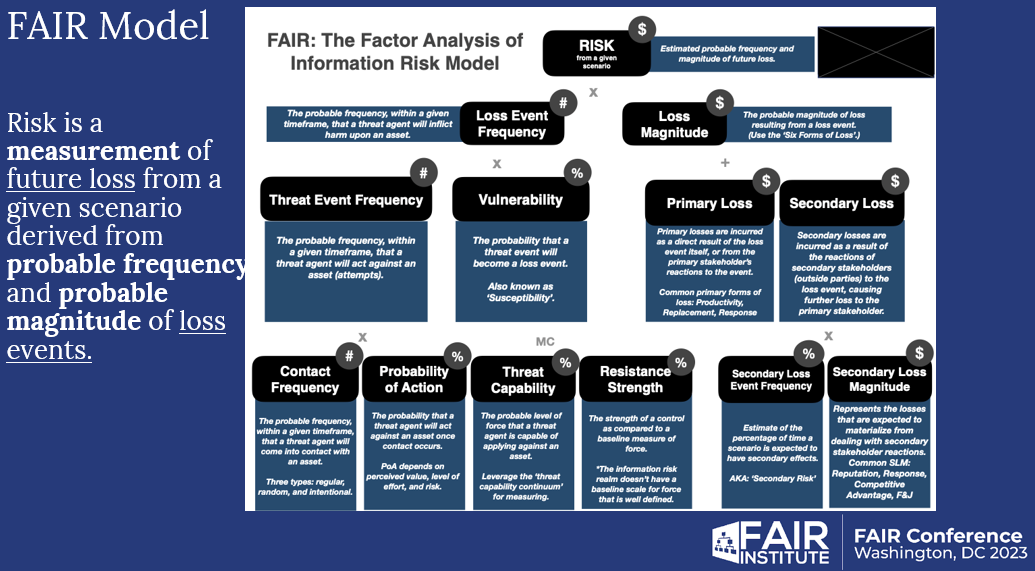
\includegraphics[width=\textwidth]{images/fair_model.png}
    \caption{FAIR (Factor Analysis of Information Risk) Model presented at FAIR Conference 2023, Washington, DC. The FAIR model is a popular implementation of CRQ.
    Credit: Jon Baker (Co-founder \& Director, Center for Threat-Informed Defense), 
    Arvin Bansal (vCISO, Fortune500), and Vidit Baxi (Co-founder \& CISO, Safe Security)}
    \label{fig:fair-model}
\end{figure}

\subsection{Testing Experience and Implementation Details}
I created a SimpleRiskModel class that implements Monte Carlo simulation to estimate 
potential losses from cyber incidents. The model was designed with these key components:
\begin{itemize}
    \item Class initialization with risk parameters (min loss, max loss, probability)
    \item Simulation method running 10,000 iterations
    \item Analysis method calculating key statistics
    \item Output formatting for clear result presentation
\end{itemize}

The testing process involved:
\begin{enumerate}
    \item Setting up a data breach scenario with realistic parameters
    \item Running multiple simulations to verify consistency
    \item Analyzing the distribution of results
    \item Validating that the average loss aligned with theoretical expectations
\end{enumerate}

Key model parameters were chosen based on typical cyber incident statistics:
\begin{itemize}
    \item Minimum loss: \$100,000 (typical small breach cost)
    \item Maximum loss: \$1,000,000 (potential major incident)
    \item Annual probability: 10\% (industry average for similar incidents)
    \item Iterations: 10,000 (for statistical significance)
\end{itemize}

\subsection{Output Examples}
\begin{verbatim}
Risk Analysis for Data Breach Scenario:
Average Annual Loss: $52,624.65
Maximum Potential Loss: $999,737.69
90th Percentile Loss: $0.00
\end{verbatim}

\subsection{Analysis}
The results show an average annual loss of about \$52,600, which aligns with the 
10\% probability of an incident occurring. The maximum potential loss approaches 
the upper limit of \$1,000,000, demonstrating the model's ability to capture 
worst-case scenarios. The 90th percentile being \$0 indicates that in most 
simulation runs (over 90\%), no loss occurred, which is consistent with the 
low probability of occurrence.

\section{Merge Conflict and Permission Resolution}
During this assignment, I encountered two significant challenges that required resolution:

\subsection{Repository Permission Issues}
Initially, I was unable to push my changes to the repository due to permission restrictions. I attempted several approaches:
\begin{enumerate}
    \item First tried pushing directly using HTTPS protocol (received 403 error)
    \item Attempted using SSH authentication
    \item Created a fork of the repository as a backup
    \item Generated a patch file (mckay-changes.patch) to preserve my changes
    \item Finally resolved when Dr. Boult granted proper repository access
\end{enumerate}

\subsection{Merge Conflicts}
After gaining proper access, I encountered merge conflicts when trying to merge upstream/main into my branch. 
The conflicts involved two files (cardenas.tex and jcastanonremy.tex) that were deleted in my branch 
but modified in upstream/main. I resolved these conflicts by:
\begin{enumerate}
    \item First checking the status using git status to understand the nature of the conflicts
    \item Using git rm --cached to remove the conflicting files from Git tracking
    \item Committing the resolution with an appropriate commit message
    \item Cleaning up the working directory by removing the untracked files
    \item Successfully completing the merge afterward
\end{enumerate}

This experience helped me understand both the importance of proper repository permissions and 
how to handle conflicts between different branches in a Git repository. It demonstrated 
real-world scenarios of collaboration challenges and their solutions.

\section{Questions and Answers}
% This section will be used later for Q&A

\end{document}
%created "images" directory in the repo. 
\section{Marwan Alharbi}

In this course, my primary goal is to delve into state-of-the-art research within the realm of wearable computing applications. I aim to identify a cutting-edge idea that aligns with my research interests and select the most relevant research papers that contribute meaningfully to this topic. By exploring the latest advancements, I hope to deepen my understanding of the current landscape in wearable computing and position my research within this innovative field.

Throughout this course, I am eager to enhance my ability to effectively search for research papers by refining my keyword selection skills. I want to learn the tips and tricks that will enable me to efficiently find the most appropriate and up-to-date research papers related to my work. Additionally, I aspire to improve my writing skills, particularly in crafting well-structured and persuasive research papers that can convince conference experts of the value and originality of my work.

\begin{figure}[h]
  \centering
  \includegraphics[width=0.30\textwidth]{images/marwan-profile.jpg}
  \caption{Marwan Alharbi, PhD student and IoT enthusiast.}
  \label{fig:marwan:profile}
\end{figure}

As a PhD student at the University of Colorado Colorado Springs (UCCS), now 
in my second year, I am committed to advancing my research in wearable 
computing. On a personal note, as a proud father of four, I balance the 
demands of family life with my academic pursuits while residing in Denver. 
In my free time, I enjoy working on IoT projects, which involve building 
printed circuit boards (PCBs) and designing 3D printed objects, including 
enclosures and moving parts. My background in web development and my 
experiments in programming languages like C/C++, Java, and Python have been 
invaluable in helping me learn algorithms and acquire skills that are 
directly applicable to my research endeavors.



\begin{figure}[h]
  \centering
  \includegraphics[width=0.90\textwidth]{images/dashboard-simulator-values.png}
  \caption{Web interface dashboard for glove sensor calibration and data management}
  \label{fig:marwan:web}
\end{figure}

\subsection{Related Implementation}
For the assignment, I chose to use my own project from the CS6770 course instead of searching for a new GitHub repository, primarily because many related GitHub projects require specialized hardware that would be difficult to acquire and test within the three-week timeframe. My project integrates several components: a glove connected to an Arduino (see Figure~\ref{fig:marwan:glove}), a controller that translates the glove's sensor data, a web interface to manage and calibrate the readings (see Figure~\ref{fig:marwan:web}), and another Arduino that controls a 3D-printed robotic finger equipped with motors to mimic the glove's movements (see Figure~\ref{fig:marwan:3d}).

\begin{figure}[h]
  \centering
  \includegraphics[width=0.80\textwidth]{images/glove-outside.png}
  \caption{Custom-made glove sensor connected to an Arduino}
  \label{fig:marwan:glove}
\end{figure}


\begin{figure}[h]
  \centering
  \includegraphics[width=0.80\textwidth]{images/physical-device.png}
  \caption{3D-printed robotic finger connected to motors and controlled by an Arduino}
  \label{fig:marwan:3d}
\end{figure}

In this implementation, I worked on hardware-software interaction, data transmission from the glove to the controller, and real-time visualization through the web interface. This approach allowed me to test the code using readily available equipment, focusing on translating the glove's readings into physical movements.

\section{Questions}
\subsection{Questions from Aaron McKay}
\begin{enumerate}
  \item In your glove sensor project, what challenges did you face in achieving accurate real-time calibration between the sensor readings and the robotic finger movements? I'm particularly interested in how you handled any latency issues in the data transmission chain.
  \subsubsection*{Answer}
  In my glove sensor project, I used a conductive sheet as a potentiometer, where bending the glove changes the sheet's resistance, producing numerical values that correspond to the finger's position. During the calibration phase, I recorded these values alongside the finger's position, and this data was mapped so the robotic finger motor could receive the correct angle based on the calibration. While there are slight errors and limitations during calibration, most of the effort ensures that the commands sent to the robotic finger are highly accurate. The data from the glove sensor is complex and requires deeper investigation to fully optimize the system.
  \item Given your background in web development and your current focus on wearable computing, how do you envision integrating edge computing principles to enhance the response time and privacy aspects of wearable devices like your sensor glove?
  
  \subsubsection*{Answer}
  With my background in web development and focus on wearable computing, I see edge computing as a way to improve response time and also help with privacy in the future. Right now, my main focus is getting accurate data from the glove sensor to control the finger movements. I have not spent much time on privacy yet, but I know it is important and something to look at later. Using edge computing can help process data directly on the glove or close to it, which reduces delays and makes the system faster. In the future, this could also help protect user privacy by keeping data local and not sending it to external servers.
\end{enumerate}



\section{Example of Easy Tables}
\csvautotabular{test.csv}


\section*{Better formated Tables}
    \begin{tabular}{r|r|r}%
    % specify table head
    \bf Time (s) & \bf Rel. time (s)& \bf Y Pos
% use head of csv as column names
    \csvreader{test.csv}{}
% specify selected coloumns here
    {\\\hline\csvcoli&\csvcolii&\csvcolvi}
    \end{tabular}
    \clearpage


\end{document}
